\documentclass[aps,prb,twocolumn,superscriptaddress,floatfix,longbibliography,10pt]{revtex4-2}

\usepackage[utf8]{inputenc}
\usepackage[spanish]{babel}
\usepackage{graphicx}
\usepackage{amsmath}
\usepackage{subcaption}
\usepackage{wrapfig} 
\usepackage[export]{adjustbox}

\usepackage{amsmath,amssymb} % math symbols
\usepackage{bm} % bold math font
\usepackage{graphicx} % for figures
\usepackage{comment} % allows block comments
\usepackage{textcomp} % This package is just to give the text quote '
%\usepackage{ulem} % allows strikeout text, e.g. \sout{text}

\usepackage[spanish]{babel}
% By dafault, spanish changes to a comma as decimal separator; to change to a dot, you can use \decimalpoint:
\decimalpoint

\usepackage{enumitem}
\setlist{noitemsep,leftmargin=*,topsep=0pt,parsep=0pt}

\usepackage{xcolor} % \textcolor{red}{text} will be red for notes
\definecolor{lightgray}{gray}{0.6}
\definecolor{medgray}{gray}{0.4}

%Para las tablas
\usepackage{multirow}

\usepackage{hyperref}
\hypersetup{
colorlinks=true,
urlcolor= blue,
citecolor=blue,
linkcolor= blue,
bookmarks=true,
bookmarksopen=false,
}

% Code to add paragraph numbers and titles
\newif\ifptitle
\newif\ifpnumber
\newcounter{para}
\newcommand\ptitle[1]{\par\refstepcounter{para}
{\ifpnumber{\noindent\textcolor{lightgray}{\textbf{\thepara}}\indent}\fi}
{\ifptitle{\textbf{[{#1}]}}\fi}}
% \ptitletrue  % comment this line to hide paragraph titles
% \pnumbertrue  % comment this line to hide paragraph numbers

% minimum font size for figures
\newcommand{\minfont}{6}

% Uncomment this line if you prefer your vectors to appear as bold letters.
% By default they will appear with arrows over them.
% \renewcommand{\vec}[1]{\bm{#1}}

%Cambiar Cuadros por Tablas y lista de...
%\renewcommand{\listtablename}{Índice de tablas}
\renewcommand{\tablename}{Tabla}
\renewcommand{\date}{Fecha}

%Para importar imágenes desde una carpeta:
\graphicspath{ {C:/Users/lupam/OneDrive/Escritorio/GitHub/Metodos_Num_Fluidos_I/Guias/Informe_final/Informe/Figures} {C:/Users/lupam/OneDrive/Escritorio/GitHub/Metodos_Num_Fluidos_I/Guias/Informe_final/Programa/graficos}}

\usepackage[bottom]{footmisc} %para que las notas al pie aparezcan en la misma página

\begin{comment}

%Comandos de interés:

* Para ordenar el documento:
\section{Introducción}
\section{\label{sec:Formatting}Formatting} %label para luego hacer referencia a esa sección

\ptitle{Start writing while you experiment} %pone nombre y título al documento dependiendo de si en el header están los comandos \ptitletrue y \pnumbertrue

* Ecuaciones:
\begin{equation}
a^2+b^2=c^2 \,.
\label{eqn:Pythagoras}
\end{equation}

* Conjunto de ecuaciones:
\begin{eqnarray}
\label{eqn:diagonal}
\nonumber d & = & \sqrt{a^2 + b^2 + c^2} \\
& = & \sqrt{3^2+4^2+12^2} = 13
\end{eqnarray}

* Para hacer items / enumerar:
\begin{enumerate}
  \item
\end{enumerate}

\begin{itemize}
  \item
\end{itemize}

* Figuras:
\begin{figure}[h]
    \includegraphics[clip=true,width=\columnwidth]{pixel-compare}
    \caption{}
     \label{fig:pixels}
\end{figure}

* Conjunto de figuras:
(no recuerdo)


* Para hacer referencias a fórmulas, tablas, secciones, ... dentro del documento:
\ref{tab:spacing}

* Para citar
Elementos de .bib
\cite{WhitesidesAdvMat2004}
url
\url{http://www.mendeley.com/}\\

* Agradecimientos:
\begin{acknowledgments}
We acknowledge advice from Jessie Zhang and Harry Pirie to produce Fig.\ \ref{fig:pixels}.
\end{acknowledgments}

* Apéndice:
\appendix
\section{\label{app:Mendeley}Mendeley}

* Bibliografía:
\bibliography{Hoffman-example-paper}

\end{comment}



\begin{document}

% Allows to rewrite the same title in the supplement
\newcommand{\mytitle}{\textcolor{red}{Título??}}

\title{\mytitle}

\author{Pablo Chehade \\
    \small \textit{pablo.chehade@ib.edu.ar} \\
    \small \textit{Métodos Numéricos en Fluidos I, Instituto Balseiro, CNEA-UNCuyo, Bariloche, Argentina, 2022} \\}


\begin{abstract}

\end{abstract}

\maketitle

\section{Introducción}

\section{Métodos Numéricos}

\section{Resultados y discusión}

\subsection{Estado estacionario}

Se calculó $u(0.5,0.5)$ y $v(0.5,0.5)$ para $Re = 1000$ y distintos dt.

\begin{figure}[h]
  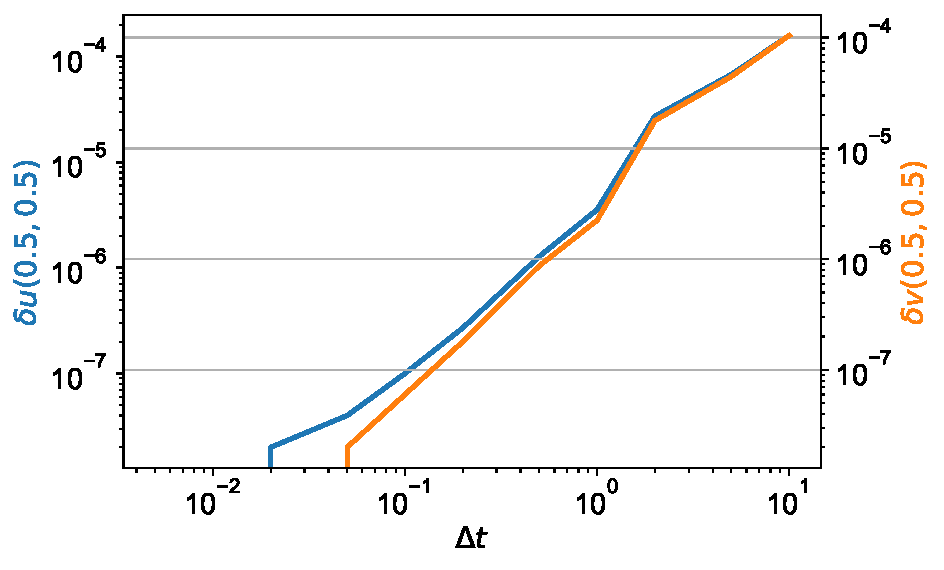
\includegraphics[clip=true,width=\columnwidth]{a_vel_vs_dt.pdf}
  \caption{}
   \label{fig:a_vel_vs_dt}
\end{figure}

Se calculó para cada caso la desviación estándar de la velocidad normalizada por el valor promedio

\subsection{Elección de dt}

\subsection{Término advectivo}

Se implementó para el término advectivo los esquemas DC2, UP1 y QUICK. Se resolvió el problema para $Re = 100, 1000 \, \mathrm{y} \, 5000$ y para $n1 = 20, 40 \, \mathrm{y} \, 80$. Se calculó para cada caso el error relativo respecto a los resultados de Guia.
$tol_estacionario = 1e-5$

\begin{figure}
  \centering
  \begin{subfigure}[b]{0.3\textwidth}
      \centering
      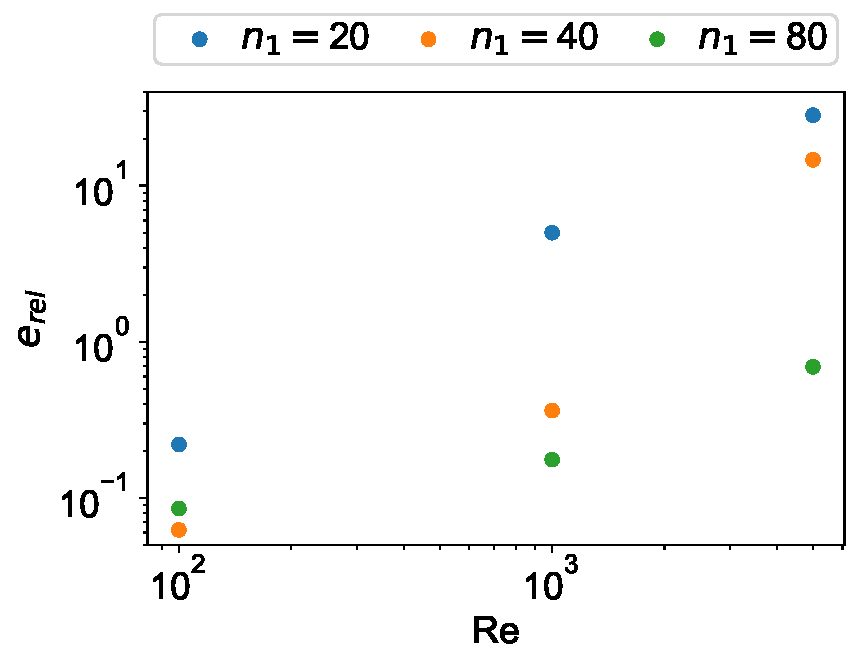
\includegraphics[width=\textwidth]{termino_adv_DC2.pdf}
      \caption{}
      \label{fig:termino_adv_DC2}
  \end{subfigure}
  \hfill
  \begin{subfigure}[b]{0.3\textwidth}
      \centering
      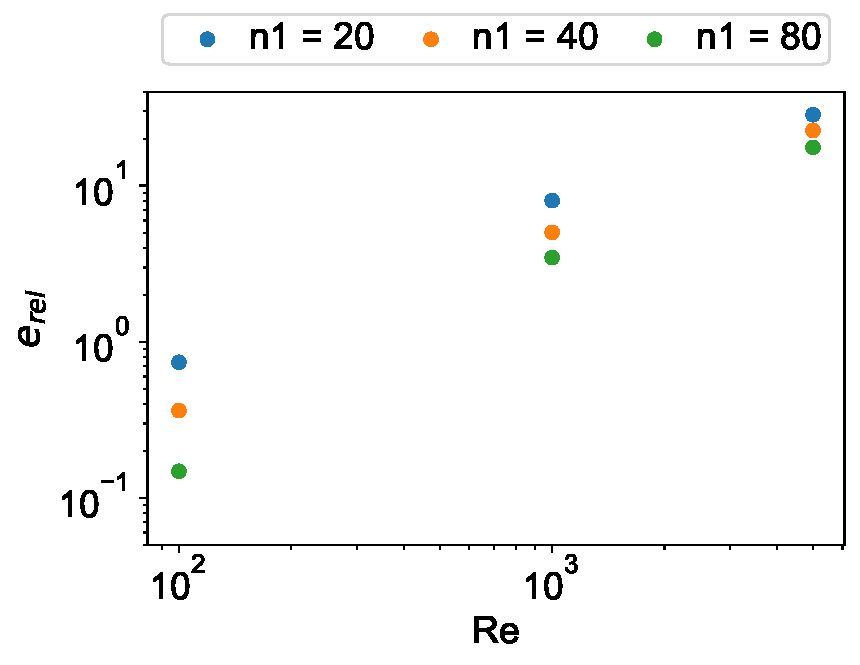
\includegraphics[width=\textwidth]{termino_adv_UP1.pdf}
      \caption{}
      \label{fig:termino_adv_UP1}
  \end{subfigure}
  \hfill
  \begin{subfigure}[b]{0.3\textwidth}
      \centering
      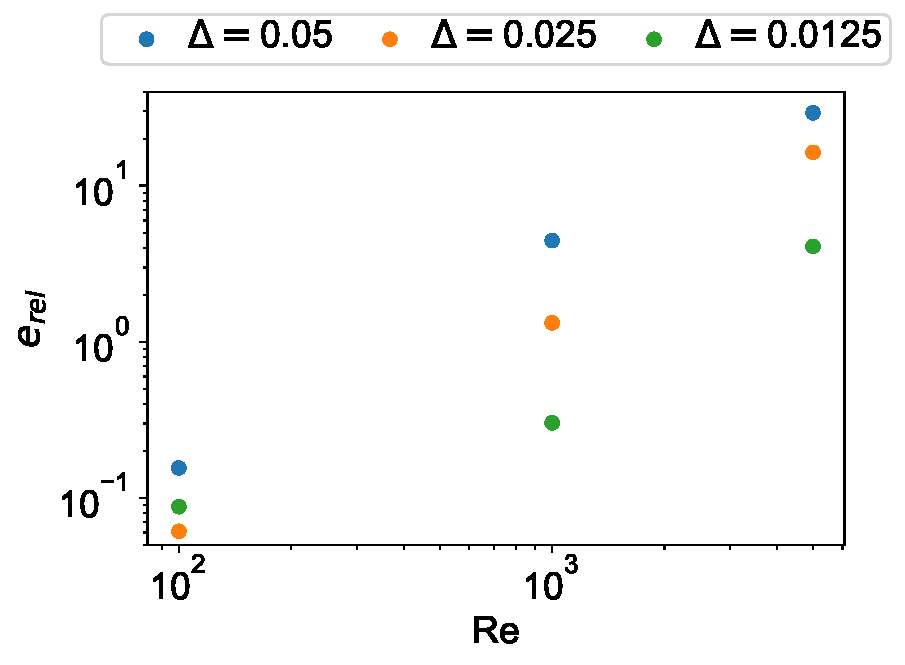
\includegraphics[width=\textwidth]{termino_adv_QUICK.pdf}
      \caption{}
      \label{fig:termino_adv_QUICK}
  \end{subfigure}
     \caption{Termino advectivo}
     \label{fig:termino_advectivo}
\end{figure}

\textcolor{blue}{Tabla con resultados}

\textcolor{red}{Duda: es necesario reportar el dt en cada caso?}

\subsection{Orden de convergencia espacial de UP1}

Se calculó $u(0.5)$ y $v(0.5)$ para $Re = 1$ y $Re = 1000$ con $n1 = 80$ y esquema QUICK. Se consideró este valor como la solución exacta. Luego, se calcularon las mismas velocidades para distintos n1 y se calculó el error respecto a la solución numérica considerada como la exacta

\begin{figure}[h]
  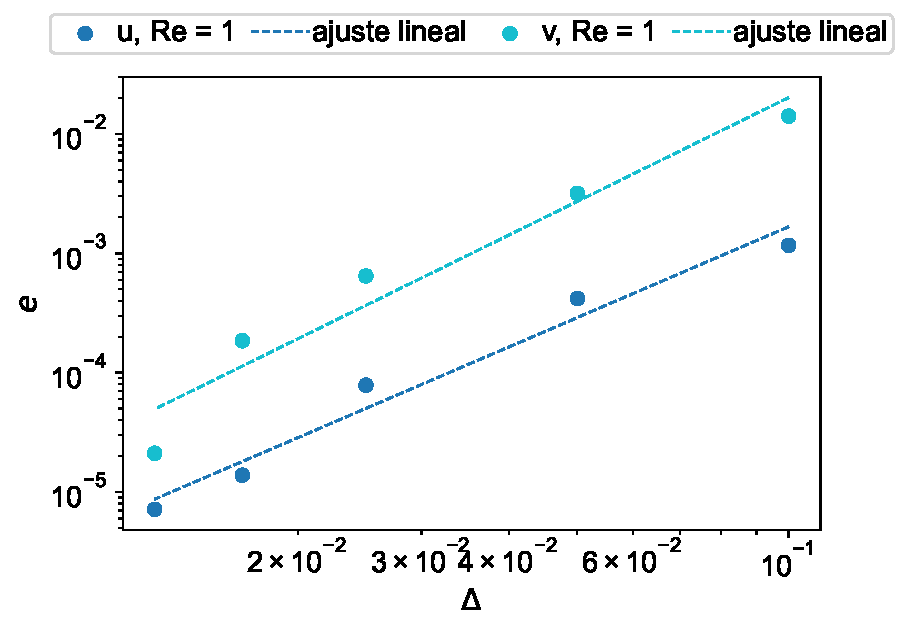
\includegraphics[clip=true,width=\columnwidth]{error_UP1_n1_vs_Re.pdf}
  \caption{}
   \label{fig:error_UP1_n1_vs_Re}
\end{figure}


\section{Conclusión}

\bibliography{Chehade_final.bib}

\end{document}





